\section{Introduction}

The Kochen--Specker (KS) theorem~\cite{KochenSpecker1967} shows that quantum observables cannot
be assigned definite values independently of the measurement context (for a review see
Ref.~\cite{Budroni2022}).  It is proved by exhibiting a finite set of rays in Hilbert space that
admits no $\{0,1\}$-valued assignment compatible with orthogonality.  Dimension three is the
smallest in which such sets exist.  (Smaller sets exist in higher dimensions, for example 20
vectors in dimension four~\cite{Kernaghan1994} and 36 in dimension
eight~\cite{KernaghanPeres1995}.)  In dimension three the smallest known set is the 31-ray
configuration of Conway and Kochen ($\CK$), reported by Peres~\cite{Peres1993}; the best lower
bound is 24, obtained for real vectors by Kirchweger, Peitl and
Szeider~\cite{KirchwegerPeitlSzeider2023} and for real and complex vectors by Li, Bright and
Ganesh~\cite{LiBrightGanesh2024}, improving the earlier 22 of Uijlen and
Westerbaan~\cite{UijlenWesterbaan2016}.  Trandafir and Cabello~\cite{TrandafirCabello2025} proved
that the orthogonality relations of $\CK$ have a unique realization up to unitary equivalence,
and that no set of 30 or fewer rays arises from one specified construction starting from the
Yu--Oh set; that 31 is the minimum without that assumption remains a conjecture.

\paragraph{The alphabet.}
Peres drew his two three-dimensional examples as cubes~\cite{Peres1991,Peres1993}: each ray joins
the centre of the cube to a marked point on its surface.  The two drawings differ in one respect.
In both, the marked points lie on a $5\times5$ grid on each face; for the 33-ray set the grid
lines sit at $0,\pm1,\pm\sqrt2$, and for $\CK$ at $0,\pm1,\pm2$ (Fig.~\ref{fig:triptych}).  The
list of coordinate values is thus a parameter of the construction, and one can ask what happens
when it is varied.  We call the list an \emph{alphabet} (Pavicic et
al.~\cite{Pavicic2019} speak of ``vector components''), a coordinate triple a \emph{word}, and the
set of all rays with coordinates in the alphabet its \emph{pool}.

\begin{figure}[t]
\centering
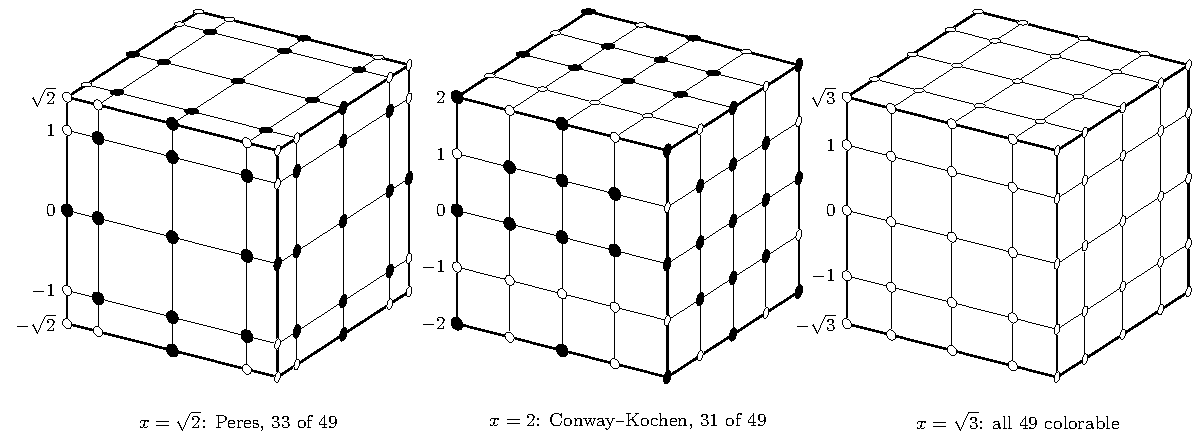
\includegraphics[width=\textwidth]{figures/alphabet_cube_triptych.pdf}
\caption{One cube, three alphabets $\{0,\pm1,\pm x\}$ with $x$ real and $x>1$.  Each of the 49
rays of the pool leaves the centre through a grid point; antipodal points are the same ray.
Filled points: the 33 rays of Peres ($x=\sqrt2$, the unique smallest uncolorable subset of that
pool) and the 31 rays of Conway and Kochen ($x=2$, one of six smallest subsets, all equivalent
under signed permutations of the axes).  At $x=\sqrt3$ the whole pool is colorable.  Only the two
inner grid lines move with~$x$.  Nearness of two points on the cube says nothing about
orthogonality of the rays, and the picture does not represent the complex pools of
Section~\ref{sec:circle}.}
\label{fig:triptych}
\end{figure}

\begin{figure}[t]
\centering
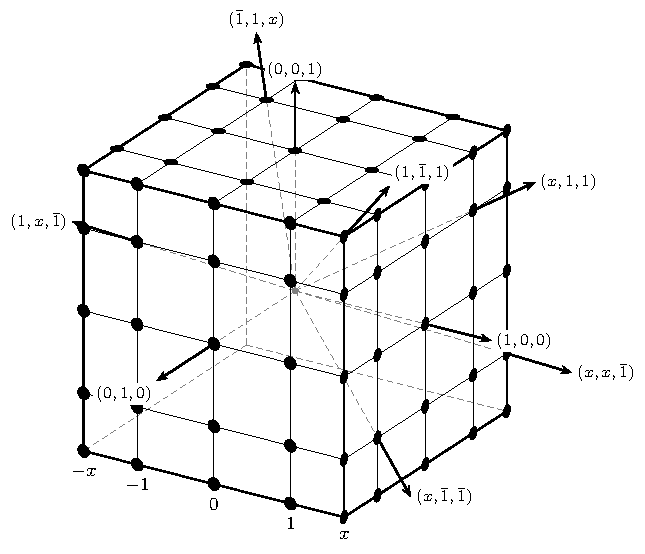
\includegraphics[width=0.6\textwidth]{figures/alphabet_cube_generic.pdf}
\caption{Words as rays.  A ray whose coordinates form a word over $\{0,\pm1,\pm x\}$ leaves the
centre of the cube $[-x,x]^3$ through a grid point; a bar is a minus sign.  Words without the
letter~$x$, such as $(1,0,0)$ and $(1,\bar1,1)$, reach the surface after scaling by~$x$.  The
49 rays are the same list of words for every~$x$; which pairs are orthogonal is not.  For
example $(x,1,1)\cdot(x,\bar1,\bar1)=x^2-1-1$, which vanishes only for $x^2=2$.}
\label{fig:generic}
\end{figure}

\paragraph{What this version claims.}
Versions 1--9 of this paper proposed that KS-uncolorability of a pool is governed by a small
number of ``cancellation mechanisms'' with a bound on the size of the generator, and that the
uncolorable alphabets form isolated ``islands''.  A full re-examination, by the author with two
language models acting as adversarial referees, found that proposal untenable: its central
statement is true by definition, its bound is contradicted by the paper's own examples, its
isolation claim is false, and one of its certified minima was wrong
(Section~\ref{sec:corrections} gives the full list).  The algorithm used to certify minima was
unsound.  Version~10 keeps the alphabet as the object of study and replaces the rest:

\begin{enumerate}[label=(\roman*)]
\item Three theorems.  Theorem~\ref{thm:twosymbol}: for every complex $x$ the pool of the
two-symbol alphabet $\{0,\pm1,\pm x\}$ is classified, and none contains a KS set of fewer than
31 rays.  Theorem~\ref{thm:6n}: the roots-of-unity pool is uncolorable exactly when
$6\mid n$.  Theorem~\ref{thm:circle}: the conjugate-closed pool over $\{0,\pm1,\pm x,\pm x^{*}\}$
is uncolorable for every $x$ on the circle $|x|^2=2$ and colorable for generic~$x$, with an
explicit smallest list of 45 words that works along the whole circle.
\item A catalogue of named finite pools (Section~\ref{sec:catalogue}), each with exact counts and
either a certified minimum KS subset or a stated upper bound, all recomputed for this version
with a certification procedure whose soundness argument is given in Section~\ref{sec:methods}.
\item A complete enumeration of the short vanishing sums available to a two-symbol alphabet
(Table~\ref{tab:zerosums}), replacing a list that had been compiled by inspection.
\end{enumerate}

Earlier versions called an uncolorable alphabet an ``island''.  Since the alphabets in question
turn out not to be isolated, this version does not use the word.

\section{Definitions and methods}\label{sec:prelim}

\begin{definition}
A \emph{ray} in $\C^3$ is a one-dimensional subspace, written $[v]$ for a nonzero vector~$v$.
Rays $[v],[w]$ are \emph{orthogonal} if $\braket vw=\sum_k v_k^{*}w_k=0$.  A \emph{triad} (or
\emph{basis}) is a set of three mutually orthogonal rays.
\end{definition}

\begin{definition}
A \emph{coloring} of a set $S$ of rays is a map $f:S\to\{0,1\}$ such that (a)~no two orthogonal
rays of $S$ both receive~1, and (b)~every triad contained in $S$ has exactly one ray with value~1.
$S$ is \emph{KS-uncolorable}, or a \emph{KS set}, if it has no coloring.  Its \emph{orthogonality
graph} has the rays as vertices and the orthogonal pairs as edges; the triads are its triangles.
Both the edges and the triangles enter the definition, and an edge lying in no triangle of $S$
is still a constraint.
\end{definition}

A coloring of $S$ restricts to a coloring of any subset, because every orthogonal pair and every
triad of the subset is one of~$S$:

\begin{lemma}[Restriction]\label{lem:restrict}
A set of rays that contains an uncolorable subset is uncolorable.
\end{lemma}

\begin{definition}
An \emph{alphabet} is a finite set $\mathcal A\subset\C$ containing~0.  Its \emph{raw pool} is
\[
S(\mathcal A)=\{\,[v]: v\in\mathcal A^3\setminus\{0\}\,\}.
\]
The \emph{completed pool} $\bar S(\mathcal A)$ is the smallest set of rays containing
$S(\mathcal A)$ and containing, with every orthogonal pair $[v],[w]$, the third ray of their
triad, $[(v\times w)^{*}]$ (the ordinary cross product for real vectors).  In all cases reported
here the completion was computed to closure and is finite; we do not know a general finiteness
criterion.
\end{definition}

In a completed pool every orthogonal pair lies in exactly one triad, so the numbers of pairs $E$
and triads $T$ satisfy $E=3T$.  This is a convenient check: the raw Eisenstein pool has
$E=174$, $T=22$, so it is not closed, contrary to a statement in version~9.

\paragraph{Three cautions on scope.}
(1)~Uncolorability is a property of a pool, not of a ring or a field.  Every ring that appears in
this paper contains $\Z$ and therefore contains the coordinates of $\CK$; the statement ``this
field supports a KS set'' is true of all of them and distinguishes nothing.  (2)~The size of a
generator is not an invariant of the pool: multiplying every word by $x^{-1}$ shows
$S(\{0,\pm1,\pm x\})=S(\{0,\pm1,\pm x^{-1}\})$, and $S$ is also unchanged by $x\mapsto-x$.
(3)~A raw pool and its completion are different objects; a statement about one says nothing about
the other, and every count below says which is meant.

\subsection{Methods}\label{sec:methods}

\paragraph{Exact arithmetic.}  Coordinates are elements of a number field $\Q[t]/(m(t))$ stored
as rational coefficient vectors; rays are compared after division by the first nonzero
coordinate; a pair is orthogonal when the Hermitian product is the zero element.  The
cyclotomic pools use exponents modulo~$n$, and the proof of Theorem~\ref{thm:circle} uses
integer polynomial identities.  No count in Sections~\ref{sec:real}--\ref{sec:catalogue} depends
on a floating-point tolerance.  The only floating-point quantities in the paper are the rigidity ranks of
Table~\ref{tab:rigidity}, including the coordinates of the 45-word set used there; they are
labelled as numerical.

\paragraph{Colorability.}  Colorability of a finite set is decided by a SAT
solver~\cite{AudemardSimon2018}: one variable per ray, a clause forbidding two 1s on each
orthogonal pair, and a clause requiring at least one 1 on each triad.

\paragraph{Certified minima.}  Let $P$ be an uncolorable pool.  If $M\subseteq P$ is colorable
then, by Lemma~\ref{lem:restrict}, every uncolorable subset of $P$ contains a ray outside~$M$.
The certifier keeps a list of such sets $M$, each verified colorable by the SAT solver, and asks
a second solver for a set $R$ of fewer than $u$ rays meeting the complement of every listed~$M$,
where $u$ is the size of the best uncolorable subset found so far.  If $R$ is uncolorable, $u$
decreases; if $R$ is colorable it is enlarged to a colorable set $M\supseteq R$ and $M$ joins the
list.  When no such $R$ exists, no uncolorable subset has fewer than $u$ rays, and the minimum is
exactly~$u$.  The answer is correct whenever the SAT solver is.  The list of sets $M$ is in principle a
certificate that can be checked independently; in this version it is archived only for
Theorem~\ref{thm:circle}, and the other minima are reproducible by re-running the scripts.  Minima that the procedure did not finish within
its time budget are reported as upper bounds.  The same enumeration, continued after the first
minimum set is found, lists \emph{all} minimum sets of a pool.

The procedure used in earlier versions (described there as ``OCUS'') was different and was not
sound: when a candidate was colorable, it required the next candidate to contain a ray that
completes a violated triad with \emph{two} rays of the current candidate, ignoring triads with
two or three rays outside it.  That can exclude genuine uncolorable subsets, and it did: it
reported 52 for the completed golden-ratio pool, which contains an uncolorable subset of~51.
None of the minima in this version comes from that code.
